\documentclass[12pt,landscape,a4paper]{article}

%%%%%% Cheatsheet Template %%%%%%%%%%%%%%
%Authors: Simon Vilmin, Johann Laconte
%%%%%%%%%%%%%%%%%%%%%%%%%%%%%%%%%%%%%%%%%

\usepackage[dvipsnames]{xcolor}
\usepackage[utf8]{inputenc}
\usepackage[english]{babel}
\usepackage[T1]{fontenc}
\usepackage{multicol}
\usepackage[top=5mm,bottom=8mm,left=8mm,right=5mm]{geometry}
\usepackage{pdfpages}
\usepackage{amsmath}
%\usepackage{amsthm}
\usepackage{array}
\usepackage{wrapfig}
\usepackage[compact]{titlesec}  % compact : no space around titles
\newcolumntype{L}[1]{>{\raggedright\let\newline\\\arraybackslash\hspace{0pt}}m{#1}}
\newcolumntype{C}[1]{>{\centering\let\newline\\\arraybackslash\hspace{0pt}}m{#1}}
\newcolumntype{R}[1]{>{\raggedleft\let\newline\\\arraybackslash\hspace{0pt}}m{#1}}

%Load colors
%from https://flatuicolors.com/
\definecolor{blueSection}{cmyk}{1,.72,0,.38}
\definecolor{blueMath}{rgb}{.17,.22,.34}
\definecolor{alizarine}{RGB}{231, 76, 60}
\definecolor{silver}{RGB}{189, 195, 199}
\definecolor{pomegranate}{RGB}{192, 57, 43}
\definecolor{midnight}{RGB}{44, 62, 80}
\definecolor{belize}{RGB}{0, 103, 176}
\definecolor{cyan}{RGB}{0, 188, 212}
\definecolor{teal}{RGB}{0, 150, 136}
\definecolor{greal}{RGB}{0, 130, 116}
\definecolor{sang}{RGB}{183, 28, 12}
\definecolor{emerald}{RGB}{0, 140, 49}
\definecolor{sunflower}{RGB}{241, 196, 15}
\definecolor{amethyst}{RGB}{155, 89, 182}
\definecolor{turquoise}{RGB}{0, 139, 128}
\definecolor{asbestos}{RGB}{127, 140, 141}
\definecolor{clouds}{RGB}{236, 240, 241}
\definecolor{lynch}{HTML}{3E4651}
\definecolor{clearsky}{HTML}{83D6DE}
\definecolor{greensea}{RGB}{22, 140, 113}
\definecolor{grass}{HTML}{97CE68}
\definecolor{peter}{RGB}{92, 192, 255}
\definecolor{lightmethyst}{RGB}{175, 109, 202}
\definecolor{pumpkin}{RGB}{211, 84, 0}
\definecolor{desire}{RGB}{181, 52, 113}
\definecolor{orangeville}{RGB}{225, 112, 85}
\definecolor{wetAsphalt}{HTML}{34495E}
\definecolor{americanRiver}{RGB}{99, 110, 114}

%%%%%%%%%%%%%%%%%%%FONTS%%%%%%%%%%%%%%%%%%%%%%%%%%%
    %change font here if needed
    \usepackage[nosf]{kpfonts}
	\usepackage[t1]{sourcesanspro}

    \DeclareMathSizes{11}{12}{9}{9}
    
%%%%%%%%%%%%%%%%%%%COLORS%%%%%%%%%%%%%%%%%%%%%%%%%%
    %set colors for math environments
    \everymath\expandafter{\the\everymath \color{blueMath}}
    \everydisplay\expandafter{\the\everydisplay \color{blueMath}}
    
    %set colors for titles
    \newcommand{\sectionColor}{pumpkin}
    \newcommand{\subsectionColor}{americanRiver}
    \newcommand{\numberingColor}{asbestos}
%%%%%%%%%%%%%%%%%%%%%%%%%%%%%%%%%%%%%%%%%%%%%%%%%%%

%compress text
\renewcommand{\baselinestretch}{.9}

%define header
\newcommand{\header}{
    \begin{tabular}{L{.2\linewidth} C{.5\linewidth} R{.25\linewidth}}
    J. Laconte &% author
    {\huge Lie Algebra for Robotics } &% Title
    
\includegraphics[height=2.5em]{cheatsheet_template/norlab_logo_acronym_dark.pdf} %logo
    \end{tabular}
    
    \noindent\textcolor{americanRiver}{\rule{\textwidth}{2pt}}
}

\pagestyle{empty}
 
%Define title styles (package titlesec) 
\titleformat{\section}[hang]
    {\bfseries}
    {\hspace{-1em} \textcolor{\numberingColor}{\thesection}\hspace{0.1em}\textcolor{asbestos}{\textbar}} % before title
    {0.2em}  % hspace
    {\bfseries\sffamily\color{pumpkin}} % title
    
\titleformat{\subsection}[hang] %subsection
    {\small\bfseries}
    {\hspace{-.6em} \textcolor{\numberingColor}{\thesubsection}\hspace{0.1em}}
    {0.2em}
    {\small\bfseries\sffamily\color{\subsectionColor}}
    
\titleformat{name=\subsection, numberless}[hang] %subsection*
    {\small\bfseries}
    {\textcolor{\numberingColor}{\textbar}}
    {0.2em}
    {\small\bfseries\sffamily\color{\subsectionColor}}

%remove some vertical space around equations and (sub)sections titles 
\AtBeginDocument{%
	\setlength\abovedisplayskip{.5em}
	\setlength\belowdisplayskip{.2em}
	\setlength\abovedisplayshortskip{-.5em}
	\setlength\belowdisplayshortskip{0em}}

%remove indent 
\setlength{\parindent}{0pt}

% %new environment for figures in multicol
\newenvironment{Figure}
  {\par\medskip\noindent\minipage{\linewidth}}
  {\endminipage\par\medskip}

%add some spacing beween the columns
\setlength\columnsep{1.5em}

\usepackage{mathtools}
\usepackage[all]{xy}

\newcommand{\R}{\mathbb{R}}
\newcommand{\I}{\mathrm{\mathbf{I}}}
\newcommand{\SO}{\mathrm{\mathbf{SO}}}
\newcommand{\SE}{\mathrm{\mathbf{SE}}}
\newcommand{\so}{\mathfrak{so}}
\newcommand{\se}{\mathfrak{se}}
\newcommand{\GL}{\mathrm{\mathbf{GL}}}
\newcommand{\vzero}{\mathbf{0}}
\newcommand{\C}{\mathbf{C}}
\newcommand{\T}{\mathbf{T}}
\newcommand{\J}{\mathbf{J}}
\newcommand{\Jc}{\mathcal{J}}

\DeclareMathOperator{\Ad}{Ad}
\DeclareMathOperator{\ad}{ad}

\begin{document}
\header
\begin{multicols*}{3}
\section{Lie Groups}
	A Lie Group is a group whose elements are organized continuously and smoothly, making it a smooth manifold.
	\subsection*{Special Orthogonal group $\SO(3)$}
		Group of 3D rotation matrix:
		$$\SO(3) = \left\{ \C \in \GL(3,\R) \,|\, \det(\C)=1, \C^T\C=\I\right\}$$%
	\subsection*{Special Euclidian group $\SE(3)$}
		Group of 3D transformation matrix:
		$$\SE(3) = \left\{ \T =%
			\begin{bmatrix}
				\C & \mathbf{r} \\
				\vzero^T & 0
			\end{bmatrix} \in \GL(4,\R)
		\,|\, \C\in\SO(3), \mathbf{r}\in\mathbb{R}^3 \right\}$$

\section{Lie algebra}
	\begin{wrapfigure}[7]{r}{.5\linewidth}
		\vskip-4em
		\centering
		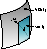
\includegraphics[width=.9\linewidth]{media/SO3.pdf}
	\end{wrapfigure}
	A Lie algebra is the tangent space of the Lie group at the identity element.
	The tangent space is defined as $ \{ \gamma'(1) \}$ where $\gamma(t)$ such that $\gamma(1) = \I$

	\subsection*{Special Orthogonal Group $\so(3)$}
		$$\so(3) = \left\{ \Phi = \phi^\wedge =%
			\begin{bmatrix}
				0 & -\phi_3 & \phi_2 \\
				\phi_3 & 0 & -\phi_1 \\
				-\phi_2 & \phi_1 & 0\\
			\end{bmatrix}
		\,|\, \phi \in \R^3 \right\}$$

		Taking the exponential of an element in $\so(3)$ leads to an element in $\SO(3)$: $\exp(\Phi) \in \SO(3)$.
		$$\Phi = \phi^\wedge \Rightarrow \phi = \Phi^\vee$$

	\subsection*{Special Euclidian Group $\se(3)$}
	$$ \se(3) = \left\{ \Xi = \xi^\wedge =
		\begin{bmatrix}
			\rho \\ \phi
		\end{bmatrix}^\wedge
		=
		\begin{bmatrix}
			\phi^\wedge & \rho \\
			\vzero^T & 0
		\end{bmatrix}
		\,|\, \rho,\phi \in \R^3
	\right\}$$

		Taking the exponential of an element in $\se(3)$ leads to an element in $\SE(3)$: $\exp(\Xi) \in \SE(3)$.
		$$\Xi = \xi^\wedge \Rightarrow \xi = \Xi^\vee$$

\section{Exponential Map}
For every square matrix $\mathbf{A}$, we have
$$\begin{aligned}
	\exp(\mathbf{A}) &= \sum_{n=0}^\infty \frac{1}{n!}\mathbf{A}^n \\
	\ln(\mathbf{A}) &= \sum_{n=1}^\infty \frac{(-1)^{n-1}}{n}(\mathbf{A}-\I)^n
\end{aligned}$$
\subsection*{Baker-Campbell-Hausdorff (BCH) formula}
Most of the time, $\exp(\mathbf{A}+\mathbf{B}) \not= \exp(\mathbf{A})\exp(\mathbf{B})$

	$$\begin{aligned} \ln(\C_1\C_2)^\vee%
	&= \phi_1 + \phi_2 + \frac12 \phi_1^\wedge\phi_2 + \cdots \\%\frac{1}{12}\phi_1^\wedge\phi_1^\wedge\phi_2 \\&+ \frac{1}{12}\phi_2^\wedge\phi_2^\wedge\phi_1 + \cdots \\
	&\approx
	\begin{cases}
		\J(\phi_2)^{-1}\phi_1 + \phi_2 \quad\text{if $\phi_1$ small} \\
		\phi_1 \J(-\phi_1)^{-1}\phi_2  \quad\text{if $\phi_2$ small}
	\end{cases}
	\end{aligned}$$

	$$\begin{aligned} \ln(\T_1\T_2)^\curlyvee%
	&= \xi_1 + \xi_2 + \frac12 \xi_1^\curlywedge\xi_2 + \cdots \\%\frac{1}{12}\xi_1^\curlywedge\xi_1^\curlywedge\xi_2 \\&+ \frac{1}{12}\xi_2^\curlywedge\xi_2^\curlywedge\xi_1 + \cdots \\
	&\approx
	\begin{cases}
		\Jc(\xi_2)^{-1}\xi_1 + \xi_2 \quad\text{if $\xi_1$ small} \\
		\xi_1 \Jc(-\xi_1)^{-1}\xi_2  \quad\text{if $\xi_2$ small}
	\end{cases}
	\end{aligned}$$

\section{Adjoints}
	The adjoint of an element of $\se(3)$ is
	$$ \ad(\Xi) = \ad(\xi^\wedge) = %
	\begin{bmatrix}
		\phi^\wedge & \rho^\wedge \\
		\vzero & \phi^\wedge
	\end{bmatrix} = 
	\xi^\curlywedge$$

	The adjoint of an element of $\SE(3)$ is
	$$ \mathcal{T} = \Ad(T) =%
	\begin{bmatrix}
		\C & \mathbf{r} \\
		\vzero & \C
	\end{bmatrix}$$
\section{Relation between spaces}
	$$\xymatrix{ 
		\phi\in\so(3) \ar[r]^\exp & \C\in\SO(3) \\
		\xi^\wedge\in\se(3) \ar[r]^\exp \ar[d]^\ad & \T\in\SE(3) \ar[d]^\Ad\\
	\xi^\curlywedge\ad(\se(3)) \ar[r]^\exp& \mathcal{T}\in\Ad(\SE(3))  }$$
	\section{(left) Jacobians}
$$\begin{aligned}
	\J(\phi) = \sum_{n=0}^\infty \frac{1}{(n+1)!} \left(\phi^\wedge\right)^n \hskip.6em 
	\Jc(\xi)= \sum_{n=0}^\infty \frac{1}{(n+1)!} \left(\xi^\wedge\right)^n 
\end{aligned}$$

\section{Interpolation}
	$$\C = (\C_2\C_1^T)^\alpha\,\C_1 \qquad \T = (\T_2\T_1^{-1})^\alpha\,\T_1$$
	with $\alpha\in[0,1]$

\section{Perturb Rotations and Poses}
	The left perturbation avoids the singularities as we stay near the identity:
	$$\C = \exp(\epsilon^\wedge)\bar{\C} \qquad \T = \exp(\varepsilon^\wedge)\bar{\T}$$
	with $\epsilon\in\R^3\sim \mathcal{N}(\vzero,\Sigma_\epsilon)$, $\varepsilon\in\R^6\sim \mathcal{N}(\vzero,\Sigma_\varepsilon)$
	\subsection{Example: Compounding poses}
	We want to find the mean and covariance of $\T=\T_1\T_2$ where $T_1=\exp(\varepsilon_1)\bar{\T}_1, T_2=\exp(\varepsilon_2)\bar{\T}_2$ and the errors $\varepsilon_1, \varepsilon_2$ have zero mean and covariances $\Sigma_1,\Sigma_2$.
	$$\begin{aligned}
		&\exp(\varepsilon^\wedge)\bar{\T} =  \exp(\varepsilon_1)\bar{\T}_1\exp(\varepsilon_2)\bar{\T}_2 \\
		\Leftrightarrow& \exp(\varepsilon^\wedge) = \exp(\varepsilon_1)\exp(\bar{\mathcal{T}}_1\varepsilon_2^\wedge) &\bar{\mathcal{T}}_1=\Ad(\bar{T}_1) \\
		\Leftrightarrow& \varepsilon = \varepsilon_1+\varepsilon_2'+\frac12\varepsilon_1^\curlywedge\varepsilon_2'+\frac{1}{12}\varepsilon_1^\curlywedge\varepsilon_1^\curlywedge\varepsilon_2' + \cdots &\varepsilon_2'=\bar{\mathcal{T}}_1\varepsilon_2
	\end{aligned}$$
	It is then possible to find $\mathbb{E}[\varepsilon]$ and $\mathbb{E}[\varepsilon\varepsilon^T]$

\end{multicols*}
\end{document}
